\newrobustcmd*{\fullfullcite}{%
    \AtNextCite{%
        \AtEachCitekey{%
            \defcounter{maxnames}{99}%
            \DeclareNameAlias{labelname}{given-family}%
        }%
    }%
    \fullcite
}

%% IMAGE AS SYMBOL

% % set the Bison QED symbol
% \renewcommand{\qed}{%
% \leavevmode\unskip\penalty9999 \hbox{}\nobreak\hfill%
% \quad\hbox{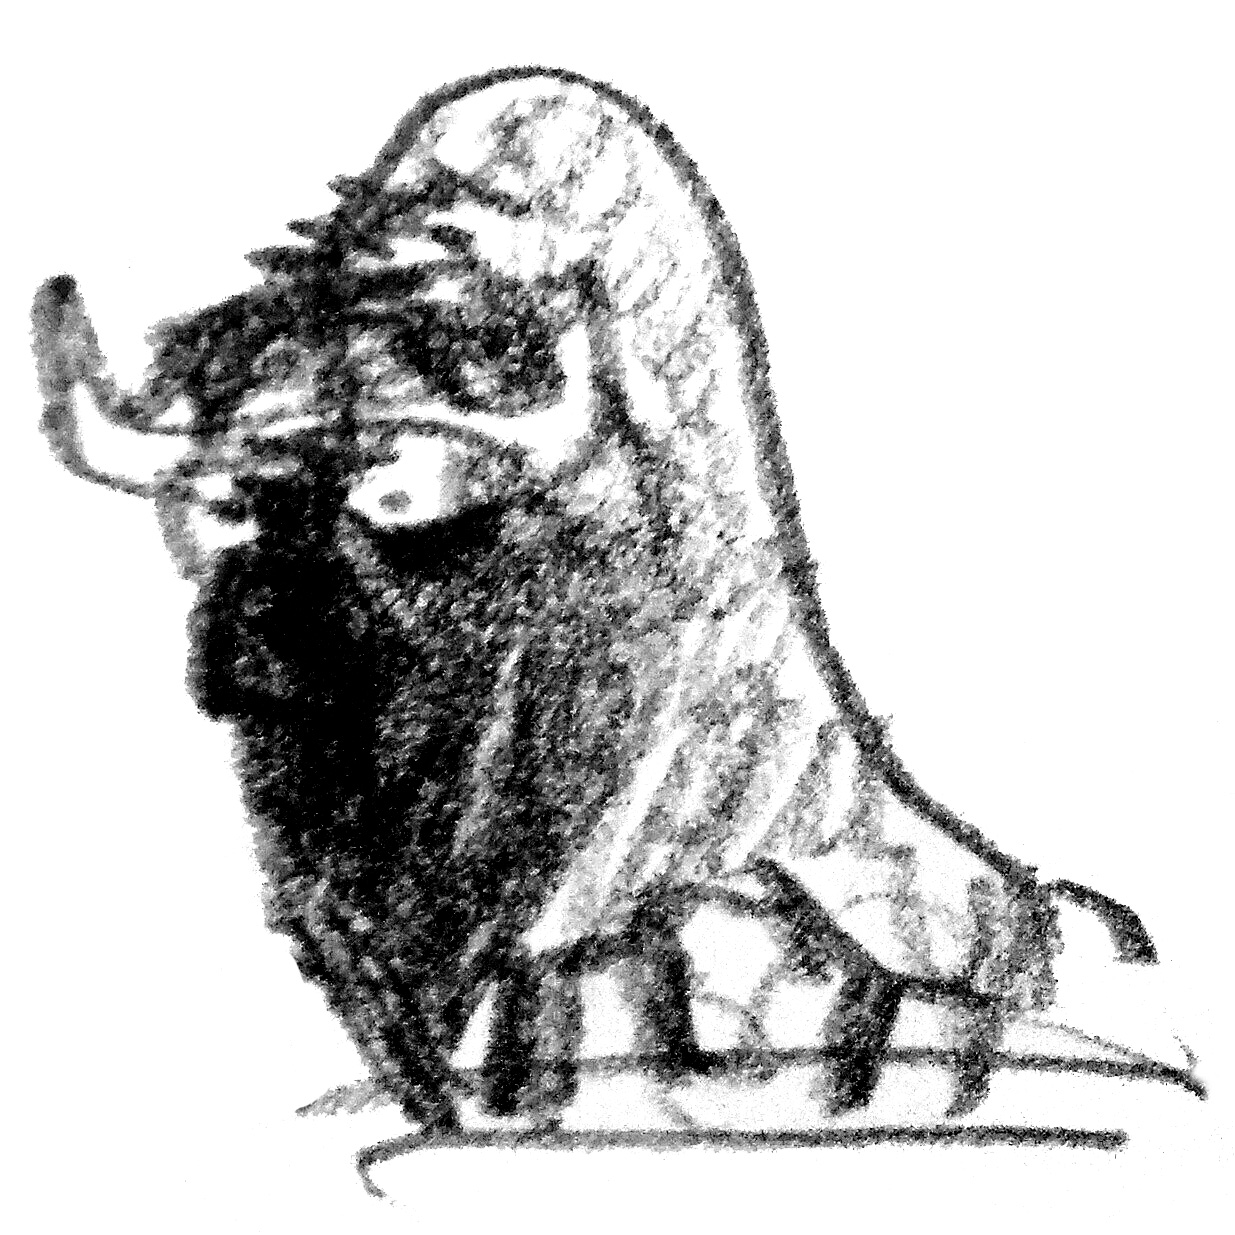
\includegraphics[height=1em]{bison/bison-qed.jpg}}}

\newcommand{\cpother}[1]{{\color{BlueGreen} #1}}
\newcommand{\cpmine}[1]{{\color{GreenYellow} #1}}

% --- my abbreviation ---------------------------------------------------------
\newcommand{\imgsrc}[1]{Image courtesy of #1}
\newcommand{\cfr}[1]{\Cf/ #1}

% --- math models -------------------------------------------------------------
\newcommand{\echoModelFreq}{\ensuremath{
    H_{ij}(f_k) = \sum_{\idxEch=0}^{\numEchs}
        \frac{\absCoeff_{ij}^r}{4 \pi \speedOfSound \tau_{ij}^r}
        \cste^{- \csti 2 \pi k \Fs \tau_{ij}^r / F}}}

\newcommand{\sumEcho}{\ensuremath{\sum_{\idxEch=0}^{\numEchs}}}
\newcommand{\echoModelTimeSimple}[1]{\ensuremath{\sumEcho \alpha_{#1}^{(r)} \delta(t - \tau_{#1}^{(r)})}}
\newcommand{\alltaus}[1]{\ensuremath{\{\tau_{#1}^{(r)}\}_{#1,r}}}
\newcommand{\allalphas}[1]{\ensuremath{\{\alpha_{#1}^{(r)}\}_{#1,r}}}

\newcommand{\icon}[1]{\raisebox{-.1\height}{\includegraphics[height=3ex]{#1}}}
\newcommand{\chaosIcon}{\icon{figures/blaster/chaos.png}}